\documentclass[9pt]{beamer}
\mode<presentation>

% Theme choice:
\usetheme{Madrid}%Darmstadt 

\usecolortheme[RGB={0,100,50}]{structure}
 \usefonttheme{structurebold} 
\setbeamercovered{invisible}
%\setbeamertemplate{navigation symbols}{}
\usepackage{dynblocks}
\usepackage{textpos}
\usepackage{amsfonts}
\usepackage{amsmath}
\usepackage{amssymb}
\usepackage{amsthm}
\usepackage{subcaption}
\usepackage{tikz}
\usetikzlibrary{arrows.meta, positioning}
\newtheorem{teorema}{Teorema}\usepackage{mathtools}
\renewcommand{\proofname}{Prova}
\usepackage[portuguese]{babel}

\uselanguage{Portuguese}
\languagepath{Portuguese}

\deftranslation[to=Portuguese]{Theorem}{Teorema}
\deftranslation[to=Portuguese]{Lemma}{Lema}
\deftranslation[to=Portuguese]{Corollary}{Corolário}
\deftranslation[to=Portuguese]{Proof}{Prova}

\usepackage{dutchcal}
\usepackage{hyperref}
\usepackage[utf8]{inputenc}
\usepackage[T1]{fontenc}
\usepackage{amsthm}


\usepackage[affil-it]{authblk} 
\usepackage{etoolbox}
\usepackage{lmodern}

\makeatletter
\patchcmd{\@maketitle}{\LARGE \@title}{\fontsize{18}{19.2}\selectfont\@title}{}{}
\makeatother

\renewcommand\Authfont{\fontsize{12}{14.4}\selectfont}
\renewcommand\Affilfont{\fontsize{9}{10.8}\itshape}

% Title page details: 
\title[Presentation]{Programação Orientada a Objetos} %add title


\institute[UniRV]{\textbf{\large  \textcolor{structure}{\textbf{\large
Encapsulamento, Métodos GET e SET, modificadores de acesso em JAVA
}} %add name 
% \hspace{0.5pt}
\\ \qquad
\\Professor: Me. Sergio Souza Novak 
\\Faculdade de Engenharia de Software}
} 
% \titlegraphic{\includegraphics[width=5cm]{msu.eps}}
\titlegraphic{
\includegraphics[width=5cm]{Universidade_de_Rio_Verde.jpg}}
\date{}

% Logo only on title page
%\logo{
\includegraphics[width=1cm,keepaspectratio]{Logo.png}}
\usepackage[pscoord]{eso-pic}


\begin{document}

% Title page frame
%\begin{frame}
    %\titlepage 
%\end{frame}
\frame[plain]{\titlepage}
%logo
\AddToShipoutPictureFG{
    \put(\LenToUnit{.92\paperwidth},
    \LenToUnit{.185\paperheight})
    {\vtop{{\null}
    \makebox{
\includegraphics[width=.8cm,keepaspectratio]{Universidade_de_Rio_Verde.jpg}}}}}


\begin{frame}{Sumário}
  \tableofcontents
\end{frame}
\begin{frame}
\setbeamercolor{background canvas}{bg=green!30!black}
\setbeamercolor{normal text}{fg=white}

\begin{center}
\vfill
{\Huge \textbf{Quando você vai se mudar,}} \\[0.5cm]
{\Huge \textbf{o que você costuma fazer}} \\[0.5cm]
{\Huge \textbf{com suas coisas?}}
\vfill
\end{center}

\end{frame}
\section{Introdução Histórica}
\begin{frame}{O Livro: A Invenção do Container}

\begin{figure}
\centering
\begin{minipage}{0.20\textwidth}
    \centering
    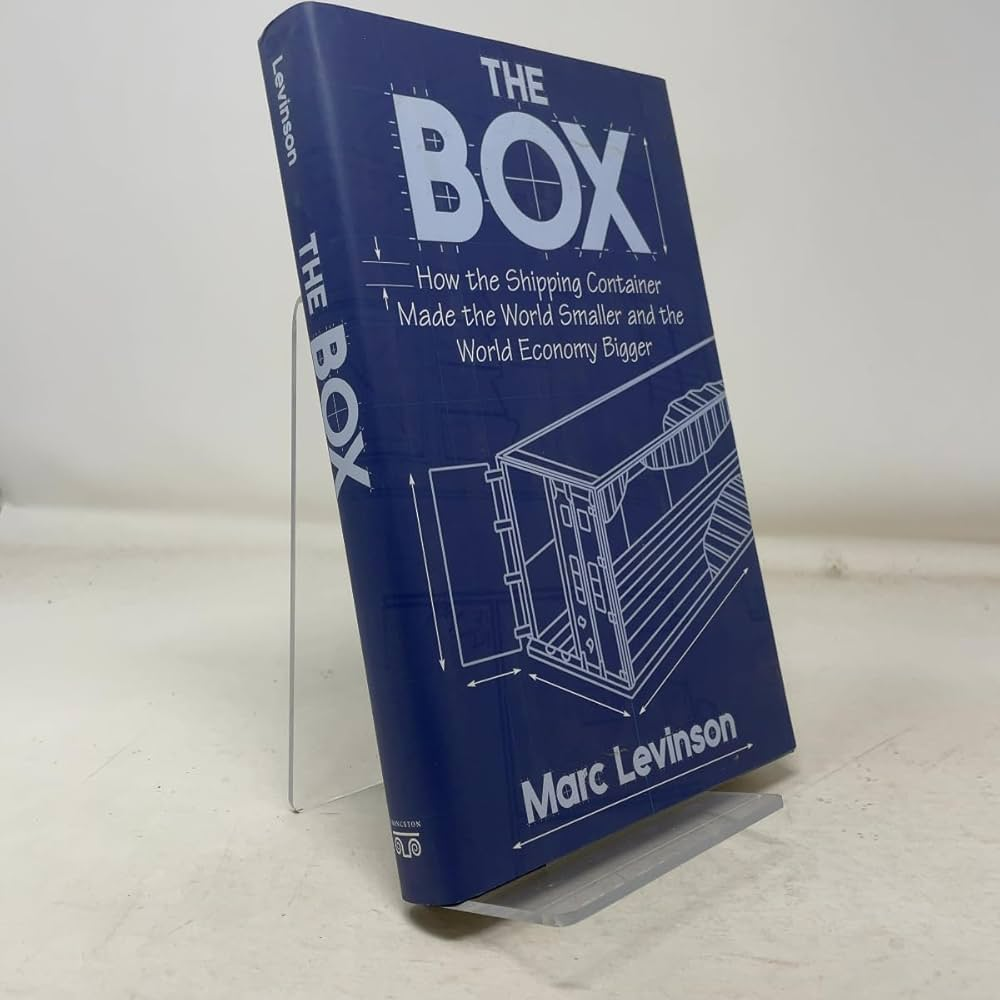
\includegraphics[width=\linewidth]{box.jpg}
    \caption{Livro "The Box" de Marc Levinson}
\end{minipage}
\hspace{0.05\textwidth}
\begin{minipage}{0.20\textwidth}
    \centering
    
\includegraphics[width=\linewidth]{box2.jpg}
    \caption{Livro "The Box" de Marc Levinson}
\end{minipage}
\end{figure}

\begin{block}{Obra}
\textbf{The Box: How the Shipping Container Made the World Smaller and the World Economy Bigger}

Autor: Marc Levinson  
Ano de publicação: 2006
\end{block}

\end{frame}
\begin{frame}{Transporte Antes da Containerização}
\begin{figure}
    \centering
    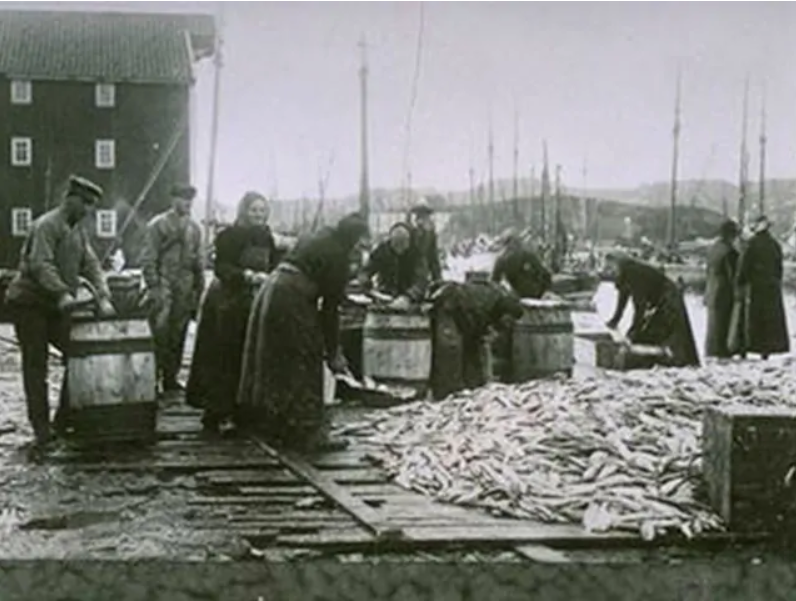
\includegraphics[width=0.75\textwidth]{mundo_sem_conteiner.png}
    \caption{Transporte global antes da padronização dos contêineres}
\end{figure}
\end{frame}

\begin{frame}{Transporte Antes da Containerização}

\begin{block}{Contexto Histórico}
Antes da padronização, as mercadorias eram transportadas manualmente
entre armazéns, navios e trens, gerando lentidão e altos custos operacionais.
\end{block}

\begin{center}
\begin{tikzpicture}[
    node distance=2cm,
    every node/.style={font=\small},
    box/.style={draw, thick, minimum width=2.8cm, minimum height=1.2cm, align=center},
    arrow/.style={-{Latex}, thick}
]

% Nodes
\node[box] (armazem) {Ponto A \\ Armazém};
\node[box, right=of armazem] (navio) {Ponto B \\ Navio};
\node[box, right=of navio] (trem) {Transporte \\ Ferroviário};

% Arrows
\draw[arrow] (armazem) -- node[above]{um a um} (navio);
\draw[arrow] (navio) -- node[above]{um a um} (trem);

% Annotation
\node[below=1.0cm of navio, align=center] 
{Exemplo: 100.000 bicicletas \\ transportadas uma a uma};

\end{tikzpicture}
\end{center}

\begin{block}{Problema Logístico}
\begin{itemize}
    \item Falta de padronização
    \item Processo lento e custoso
    \item Elevado esforço humano
    \item Gargalos nos portos
\end{itemize}
\end{block}

\end{frame}

\begin{frame}{O Livro: A Invenção do Container}

\begin{block}{Tema Central}
A obra analisa como a padronização do transporte por contêiner
transformou radicalmente:
\begin{itemize}
    \item O comércio internacional
    \item A logística global
    \item A organização das cadeias produtivas
\end{itemize}
\end{block}
\end{frame}
\begin{frame}{Container vs Encapsulamento em Objetos}

\centering
\begin{tikzpicture}[
    node distance=1.8cm,
    box/.style={draw, thick, minimum width=3.5cm, minimum height=2.5cm, align=center},
    benefit/.style={draw, rounded corners, align=left, font=\small},
    >=Stealth
]

% --- Container físico ---
\node[box] (container) {
\textbf{CONTAINER}\\
\rule{3cm}{0.8pt}\\
Carga protegida\\
Padronização\\
Transporte intermodal
};

\node[benefit, below=of container] (benefc) {
\textbf{Benefícios:}\\
$\bullet$ Padronização logística\\
$\bullet$ Redução de custos\\
$\bullet$ Agilidade operacional\\
$\bullet$ Segurança da carga
};

% --- Encapsulamento ---
\node[box, right=4.5cm of container] (objeto) {
\textbf{OBJETO}\\
\rule{3cm}{0.8pt}\\
Atributos\\
Métodos\\
Interface pública
};

\node[benefit, below=of objeto] (benefo) {
\textbf{Benefícios:}\\
$\bullet$ Ocultação de dados\\
$\bullet$ Redução de acoplamento\\
$\bullet$ Manutenção facilitada\\
$\bullet$ Reuso de código
};

% --- Setas comparativas ---
\draw[<->, thick] (container) -- node[above]{Proteção e Organização} (objeto);

\end{tikzpicture}

\vspace{0.4cm}

\begin{block}{Analogia Estrutural}
O container encapsula mercadorias para transporte eficiente.  
O objeto encapsula dados e comportamentos para organização e segurança do sistema.
\end{block}

\end{frame}
\section{Encapsulamento: Definição e Importância}
\section{Encapsulamento}

\begin{frame}{Encapsulamento em Orientação a Objetos}

\begin{block}{Definição}
O \textbf{Encapsulamento} é um dos pilares da Orientação a Objetos e consiste no
\textbf{princípio de ocultar os detalhes internos de implementação de uma classe},
permitindo acesso controlado aos seus dados.
\end{block}

\begin{block}{Objetivo}
\begin{itemize}
    \item Proteger o estado interno do objeto
    \item Garantir integridade dos dados
    \item Controlar como os atributos são modificados
\end{itemize}
\end{block}

\begin{block}{Ideia Central}
O acesso direto aos atributos deve ser evitado,
sendo realizado por meio de métodos públicos controlados.
\end{block}

\end{frame}
\begin{frame}{Modificadores de Acesso em Java}

\begin{block}{Principais Modificadores}
\begin{itemize}
    \item \textbf{public} → acesso livre
    \item \textbf{private} → acesso restrito à própria classe
    \item \textbf{protected} → acesso na mesma classe, pacote ou subclasses
    \item \textbf{default} → acesso apenas dentro do pacote
\end{itemize}
\end{block}

\begin{block}{Encapsulamento na Prática}
Para aplicar encapsulamento:
\begin{itemize}
    \item Declarar atributos como \texttt{private}
    \item Criar métodos públicos de acesso
\end{itemize}
\end{block}

\end{frame}

\begin{frame}{Modificador \texttt{public}}

\begin{block}{Onde é aplicado}
Classes, atributos, métodos e construtores.
\end{block}

\begin{block}{Função}
Permite acesso a partir de qualquer classe,
independentemente do pacote.
\end{block}

\begin{block}{Uso típico}
Define a interface pública do objeto.
\end{block}

\end{frame}
\begin{frame}[fragile]{Exemplo com \texttt{public}}

\begin{verbatim}
public class Camera {

    public String marca;

    public void ligar() {
        System.out.println("Ligando camera");
    }
}
\end{verbatim}

\end{frame}

\begin{frame}[fragile]{Invocação com \texttt{public}}

\begin{verbatim}
Camera c = new Camera();

c.marca = "Canon";      // POSSÍVEL
c.ligar();              // POSSÍVEL
\end{verbatim}

\begin{block}{Observação}
Pode ser acessado de qualquer classe.
\end{block}

\end{frame}

\begin{frame}{Modificador \texttt{private}}

\begin{block}{Onde é aplicado}
Atributos, métodos e construtores.
\end{block}

\begin{block}{Função}
Restringe o acesso exclusivamente à própria classe.
\end{block}

\begin{block}{Objetivo}
Implementar encapsulamento e proteção de estado.
\end{block}

\end{frame}

\begin{frame}[fragile]{Exemplo com \texttt{private}}

\begin{verbatim}
public class Camera {

    private String modelo;

    private void resetar() {
        System.out.println("Resetando...");
    }

    public String getModelo() {
        return modelo;
    }
}
\end{verbatim}

\end{frame}
\begin{frame}[fragile]{Invocação com \texttt{private}}

\begin{verbatim}
Camera c = new Camera();

c.modelo = "X100";      // IMPOSSÍVEL
c.resetar();            // IMPOSSÍVEL
c.getModelo();          // POSSÍVEL
\end{verbatim}

\begin{block}{Observação}
Acesso somente por métodos públicos da própria classe.
\end{block}

\end{frame}
\begin{frame}{Modificador \texttt{protected}}

\begin{block}{Onde é aplicado}
Atributos, métodos e construtores.
\end{block}

\begin{block}{Função}
Permite acesso:
\begin{itemize}
\item Na própria classe
\item No mesmo pacote
\item Em subclasses (mesmo em pacotes diferentes)
\end{itemize}
\end{block}

\end{frame}
\begin{frame}{Modificador \texttt{protected}}

\begin{block}{Onde é aplicado}
Atributos, métodos e construtores.
\end{block}

\begin{block}{Função}
Permite acesso:
\begin{itemize}
\item Na própria classe
\item No mesmo pacote
\item Em subclasses (mesmo em pacotes diferentes)
\end{itemize}
\end{block}

\end{frame}
\begin{frame}[fragile]{Invocação com \texttt{protected}}

\begin{verbatim}
Camera c = new Camera();

c.resolucao = 20;   // IMPOSSÍVEL fora do pacote
c.configurar();     // IMPOSSÍVEL fora do pacote
\end{verbatim}

\begin{block}{Observação}
Acesso permitido em subclasses e mesmo pacote.
\end{block}

\end{frame}
\begin{frame}{Modificador \texttt{default}}

\begin{block}{Onde é aplicado}
Classes (sem modificador), atributos e métodos.
\end{block}

\begin{block}{Função}
Permite acesso apenas dentro do mesmo pacote.
\end{block}

\begin{block}{Importante}
É o modificador padrão quando nenhum é declarado.
\end{block}

\end{frame}
\begin{frame}[fragile]{Exemplo com \texttt{default}}

\begin{verbatim}
class Camera {

    String modelo;      // default

    void ligar() {      // default
        System.out.println("Ligando...");
    }
}
\end{verbatim}

\end{frame}
\begin{frame}[fragile]{Exemplo com \texttt{default}}

\begin{verbatim}
class Camera {

    String modelo;      // default

    void ligar() {      // default
        System.out.println("Ligando...");
    }
}
\end{verbatim}

\end{frame}

\begin{frame}[fragile]{Exemplo Sem Encapsulamento}

\begin{verbatim}
public class ContaBancaria {
    public double saldo;
}
\end{verbatim}

\begin{block}{Problema}
O atributo \texttt{saldo} pode ser alterado diretamente:

\begin{verbatim}
conta.saldo = -1000;
\end{verbatim}

Isso compromete a integridade do objeto.
\end{block}

\end{frame}
\begin{frame}[fragile]{Aplicando Encapsulamento}

\begin{verbatim}
public class ContaBancaria {

    private double saldo;

    public void depositar(double valor) {
        if (valor > 0) {
            saldo += valor;
        }
    }

    public double getSaldo() {
        return saldo;
    }
}
\end{verbatim}

\begin{block}{Análise Técnica}
\begin{itemize}
    \item O atributo \texttt{saldo} é privado
    \item A modificação ocorre apenas por métodos controlados
    \item Regras de negócio podem ser implementadas
\end{itemize}
\end{block}

\end{frame}
\begin{frame}{Classe CameraDigital}
\begin{figure}
    \centering
    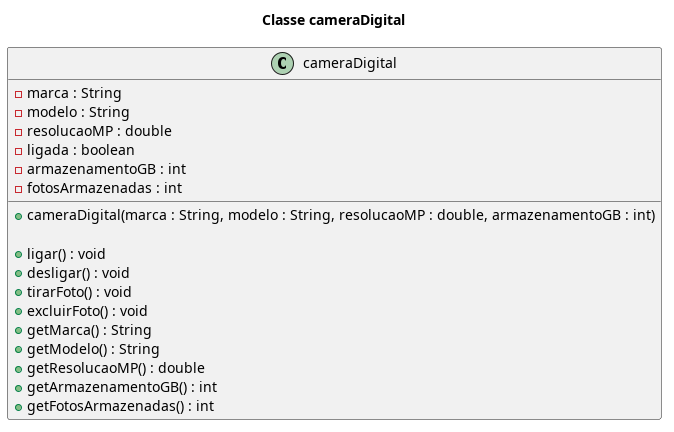
\includegraphics[width=0.9\textwidth]{cameraDigital.png}
    \caption{Diagrama de classe da classe CameraDigital}
\end{figure}
\end{frame}
\begin{frame}{Classe CameraDigital}
\begin{figure}
    \centering
    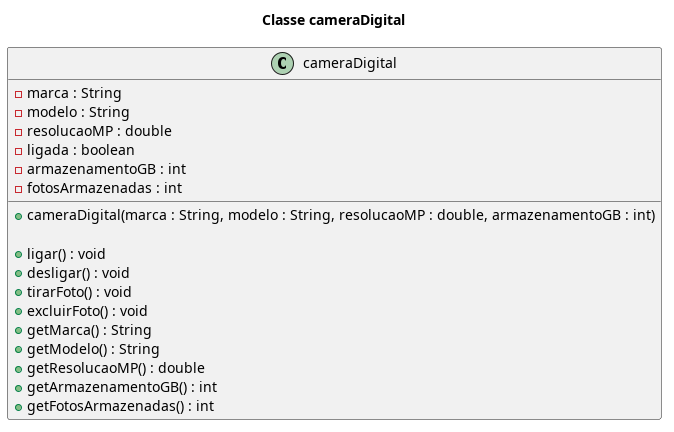
\includegraphics[width=0.5\textwidth]{cameraDigital.png}
    \caption{Diagrama de classe da classe CameraDigital}
\end{figure}
\begin{block}{Análise Técnica}
\begin{itemize}
    \item Atributos privados: \texttt{resolucao}, \texttt{zoom}, \texttt{ligada}
    \item Métodos públicos: \texttt{tirarFoto()}, \texttt{ligar()}, \texttt{desligar()}
    \item Encapsulamento protege o estado interno da câmera
    \item Interface pública controla o comportamento da câmera.
\end{itemize}
\end{block}
\end{frame}
\section{Método GET}

\begin{frame}{Método GET}

\begin{block}{Onde é aplicado}
\begin{itemize}
    \item Em classes que utilizam encapsulamento
    \item Para acessar atributos privados
\end{itemize}
\end{block}

\begin{block}{Função}
\begin{itemize}
    \item Retornar o valor de um atributo
    \item Permitir leitura controlada do estado do objeto
\end{itemize}
\end{block}

\begin{block}{Características}
\begin{itemize}
    \item Geralmente público
    \item Não recebe parâmetros
    \item Retorna o tipo do atributo
\end{itemize}
\end{block}

\end{frame}
\begin{frame}[fragile]{Exemplo de Método GET}

\begin{verbatim}
public class Camera {

    private String modelo;

    public String getModelo() {
        return modelo;
    }
}
\end{verbatim}

\begin{block}{Invocação}
\begin{verbatim}
Camera c = new Camera();
String m = c.getModelo();  // leitura permitida
\end{verbatim}
\end{block}
\end{frame}

\section{Método SET}
\begin{frame}{Método SET}

\begin{block}{Onde é aplicado}
\begin{itemize}
    \item Em classes com atributos privados
    \item Para modificar valores internos
\end{itemize}
\end{block}

\begin{block}{Função}
\begin{itemize}
    \item Alterar o valor de um atributo
    \item Permitir escrita controlada
\end{itemize}
\end{block}

\begin{block}{Características}
\begin{itemize}
    \item Geralmente público
    \item Recebe um parâmetro
    \item Retorna \texttt{void}
\end{itemize}
\end{block}

\end{frame}
\begin{frame}[fragile]{Exemplo de Método SET com Validação}

\begin{verbatim}
public class Camera {

    private String modelo;

    public void setModelo(String modelo) {
        if (modelo == null || modelo.trim().isEmpty()) {
            throw new IllegalArgumentException(
                "O modelo não pode ser vazio."
            );
        }
        this.modelo = modelo;
    }
}
\end{verbatim}

\begin{block}{Invocação}
\begin{verbatim}
Camera c = new Camera();
c.setModelo("Canon");   // válido

c.setModelo("");        // lança exceção
c.setModelo(null);      // lança exceção
\end{verbatim}
\end{block}

\end{frame}
\begin{frame}{Mensagem final}
\begin{figure}[h]
\centering
\begin{minipage}{0.20\textwidth}
    \centering
    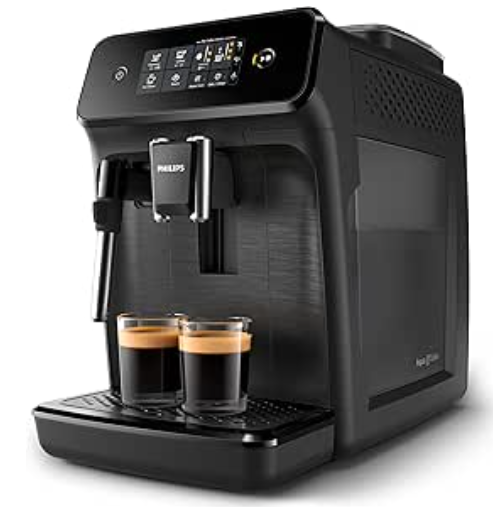
\includegraphics[width=\linewidth]{cafeteira.png}
\end{minipage}
\hspace{0.05\textwidth}
\begin{minipage}{0.20\textwidth}
    \centering
    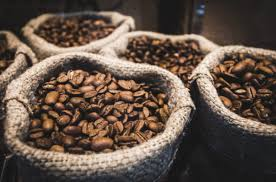
\includegraphics[width=\linewidth]{cafe_commodity.jpeg}
\end{minipage}

\caption{Cafeteira como exemplo de encapsulamento e café como commodity transportável.}
\end{figure}

\end{frame} 


\end{document}
